\section{Interpolation}
Zu gegebenen Punkten $ ( x_{i}, y_{i} ), i=0, ..., n $ mit $ x_{i} \neq x_{j} $ für $ i \neq  j $ eine Funktion G ( dies ist nicht eindeutig! Abhängig von der Funktionsklasse ), so dass $ G ( x_{i} ) = y_{i}, i=0, ..., n $ (Interpolationsbedingung). Interpolation ist \textbf{ungeeignet} für verauschte Daten. Lösung: Approximation der kleinsten Quadrate.

\subsection{Begriffe}
Extrapolation $\hat{=} $ Näherungwerte für x-Werte außerhalb der Stützstellen;\\
Dividierende Differenzen $\hat{=}$ Koeffizienten $ c_{i} $ lassen sich rekursiv durch wiederholte Bildung von "Differenzquotienten" berechnen
\subsection{Vandermonde/klassisch}
Unterschiedliche Darstellungen für ein Interpolationspolynom $ G(x) = p_{n}(x) $ vom Grad $ n $ haben unterschiedliche Eigenschaften bei der numerischen Berechnung.\textbf{Monombasis:} $ x^{0}, x^{1}, x^{2}, x^{3}, ...; p_{n}(x) = a_{n} x^n + ... + a_{1} x^{1} + a_{0} x^{0} $; 
\textbf{Ziel:} Bestimmung d. Koeffizienten $ a_{0}, a_{1}, ..., a_{n} $ sodass $ p_{n}( x_{i} ) = y_{i} = a_{n} x_{i}^n + ... + a_{1} x_{i}^1 +a_{0} x^{0} $ für i = 0, ..., n; 
\textbf{Für die eindeutige Lösung n+1 Gleichungen: Interpolationsbedingungen};
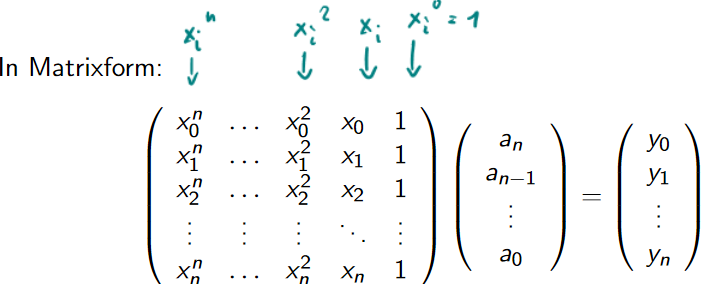
\includegraphics[scale=0.25]{./pic/VandermondeMatrix.png}
Die Koeffizientenmatrix ist die sog. \textbf{Vandermonde Matrix}; \textbf{Eigenschaften:} Die Vandermonde Matrix ist nicht singulär( falls alle $ x_{i} $ verschieden); Rechenaufwand: $ \mathcal O ( n^{3} ) $; Für große n sehr schlecht konditioniert \& als Allgemeiner Ansatz ungeeignet.

\subsection{Lagrange}
\textbf{2 Formeln}; 
$ p_{n}(x) = y_{0} L_{0} (x) + y_{1} L_{1} (x)+ ... +y_{n} L_{n} (x) $;
$ L_{k}(x) \prod_{ j = 0;j\neq k }^{n} \frac{ x-x_{j} }{ x_{k} - y_{j} } $; 
Jede Basisfunktion $ L_{k}(x) $ ist ein Polynom vom Grad $ \le n $; 
\textbf{Bemerkung:} Findet Anwendung bei Numerischer Integration; Wenn Stützstellen $ x_{i}  $ gleich bleiben \& nur $ y_{i} $ ändern $ \Rightarrow $ keine Neuberechnung; Rechenaufwand $ \mathcal O ( ( n +1)^{2} ) $; Kommen neue Stützpunkte hinzu $ \Rightarrow $ Neuberechnung\textbf{!}; Die Interpolationspolynome liefern nur sinnvolle \textbf{ Näherungswerte } für x-Werte, die zwischen den gegebenen Stützstellen liegen; Extrapolation ( Näherungwerte für x-Werte außerhalb der Stützstellen ) kann zu großen Abweichungen führen.

\subsection{Newton}
Darstellung des Interpolanten, die auf ein gestaffeltes LGS führt \& einfache Hinzunahme weiterer Punkte erlaubt.
$p_{n}(x) = c_{0} + c_{1} ( x-x_{0} ) + ... + \underbrace {c_{n} ( x-x_{0} ) ( x-x_{1} ) ... ( x-x_{n-1} ) } $\\
Polynom vom Grad n\\
Das Resultierende LGS für die Koeffizienten $ c_{i} $ hat gestaffelte Form.
\textbf{Interpolationsbedingungen?}\\
\textbf{Vorteile:} Rechenaufwand $ \mathcal O ( n^{2} ) $ Gleitpunktoperationen; Hinzufügen weiterer Stützstellen ohne großen Aufwand. Andere Koeffizienten bleiben unverändert.

\subsection{Dividierende Differenzen}
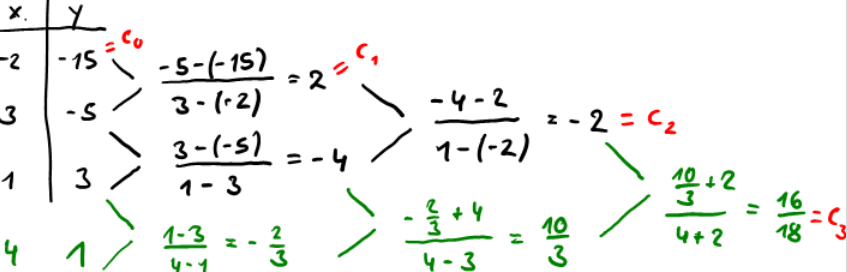
\includegraphics[scale=0.25]{./pic/DividierendeDifferenzen.png}

\subsection{Effizienz}
\subsubsection{klasisch}
$ p_{n} (x) = a_{n} x^{n} + ... + a_{0} $; 
\textbf{Aufwand:} 2n-1 Mult.
\subsubsection{Horner Schema}
$ p_{3} (x) = a_{3} x^{3} + a_{2} x^{2} + a_{1} + a_{0} = (( a_{3} + a_{2} ) x + a_{1} )x+ a_{0} $; 
Allg.: $ p_{n} (x) = ( ... ( a_{n} x + a_{n-1} ) x + ... + a_{1} ) x + a_{0} $; 
\textbf{Aufwand:} n Mult.

\subsection{Interpolationsfehler}
Falls $ f $ hinreichend glatt ist \& $ p_{n} $ das eindeutige Interpolationspolynom von Gradn $ n $, dann gilt fürn den Interpolationsfehler:
$ f(x) - p_{n}(x) = \underbrace{ \frac{ f^{ ( n+1 ) }( \theta ) }{ ( n+1) ! } ( x-x_{0} )...( x-x_{n} ) } $ mit $ \theta \in [ x_{0}; x_{n} ]  $\\
Vergleichbar zum Restglied bei der Taylorreihenentwicklung; 
\textbf{Bemerkung:} $ \theta $ unbekannt, daher nur Fehlerabschätzung; 
Fehler ist Abhängig von der Verteilung der Stützstellen; 
Der Fehler ist bei großen n an den Intervallrändern deutlich größer, als in der Intervallmitte
\subsubsection{Wahl der Stüztstellen}
Runge Funktion $ (f) $